\begin{figure}[htbp]
\centering
\begin{tabular}{ccc}
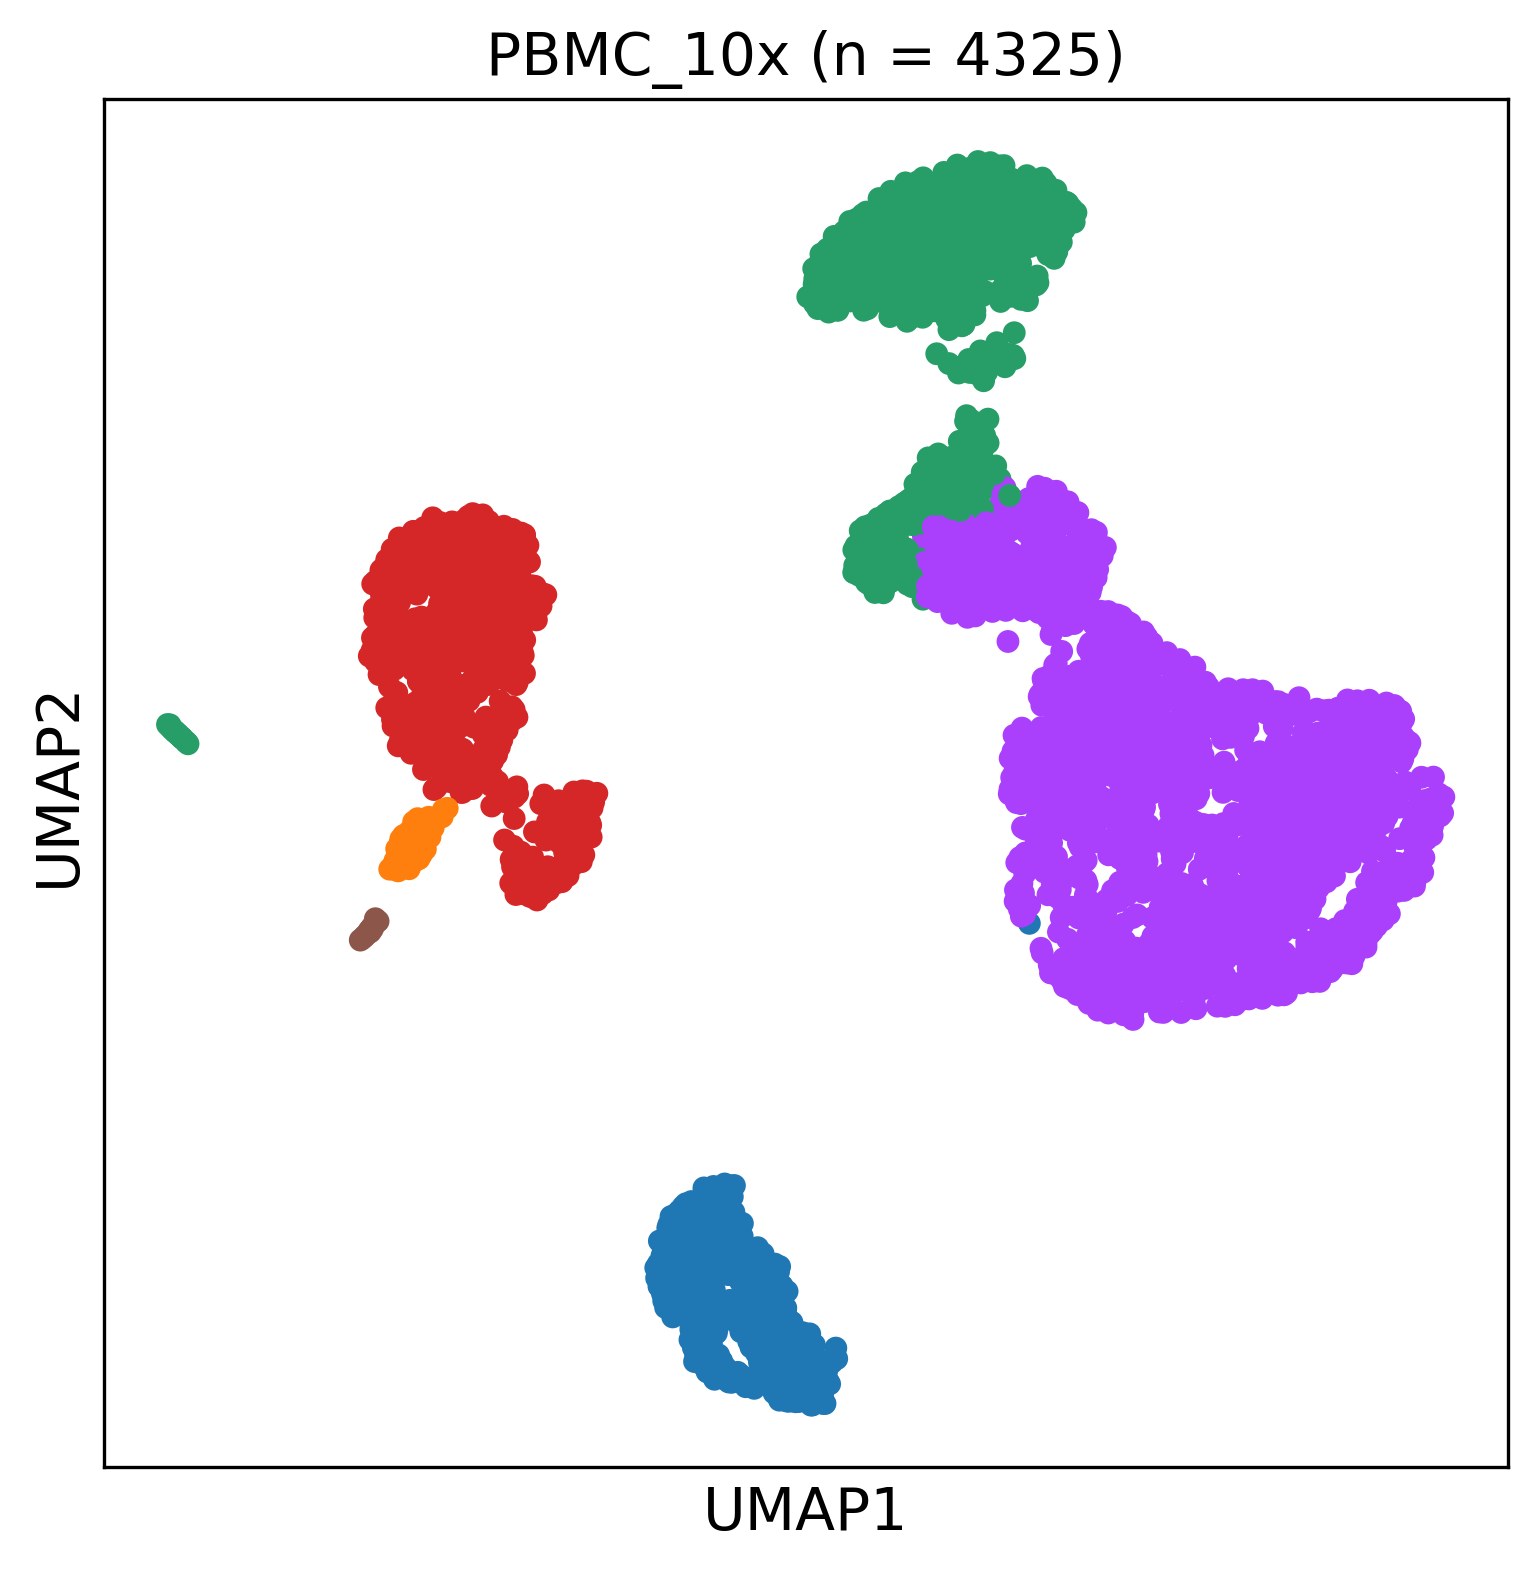
\includegraphics[width=0.25\textwidth]{images/clusterings/PBMC_10x.png} &
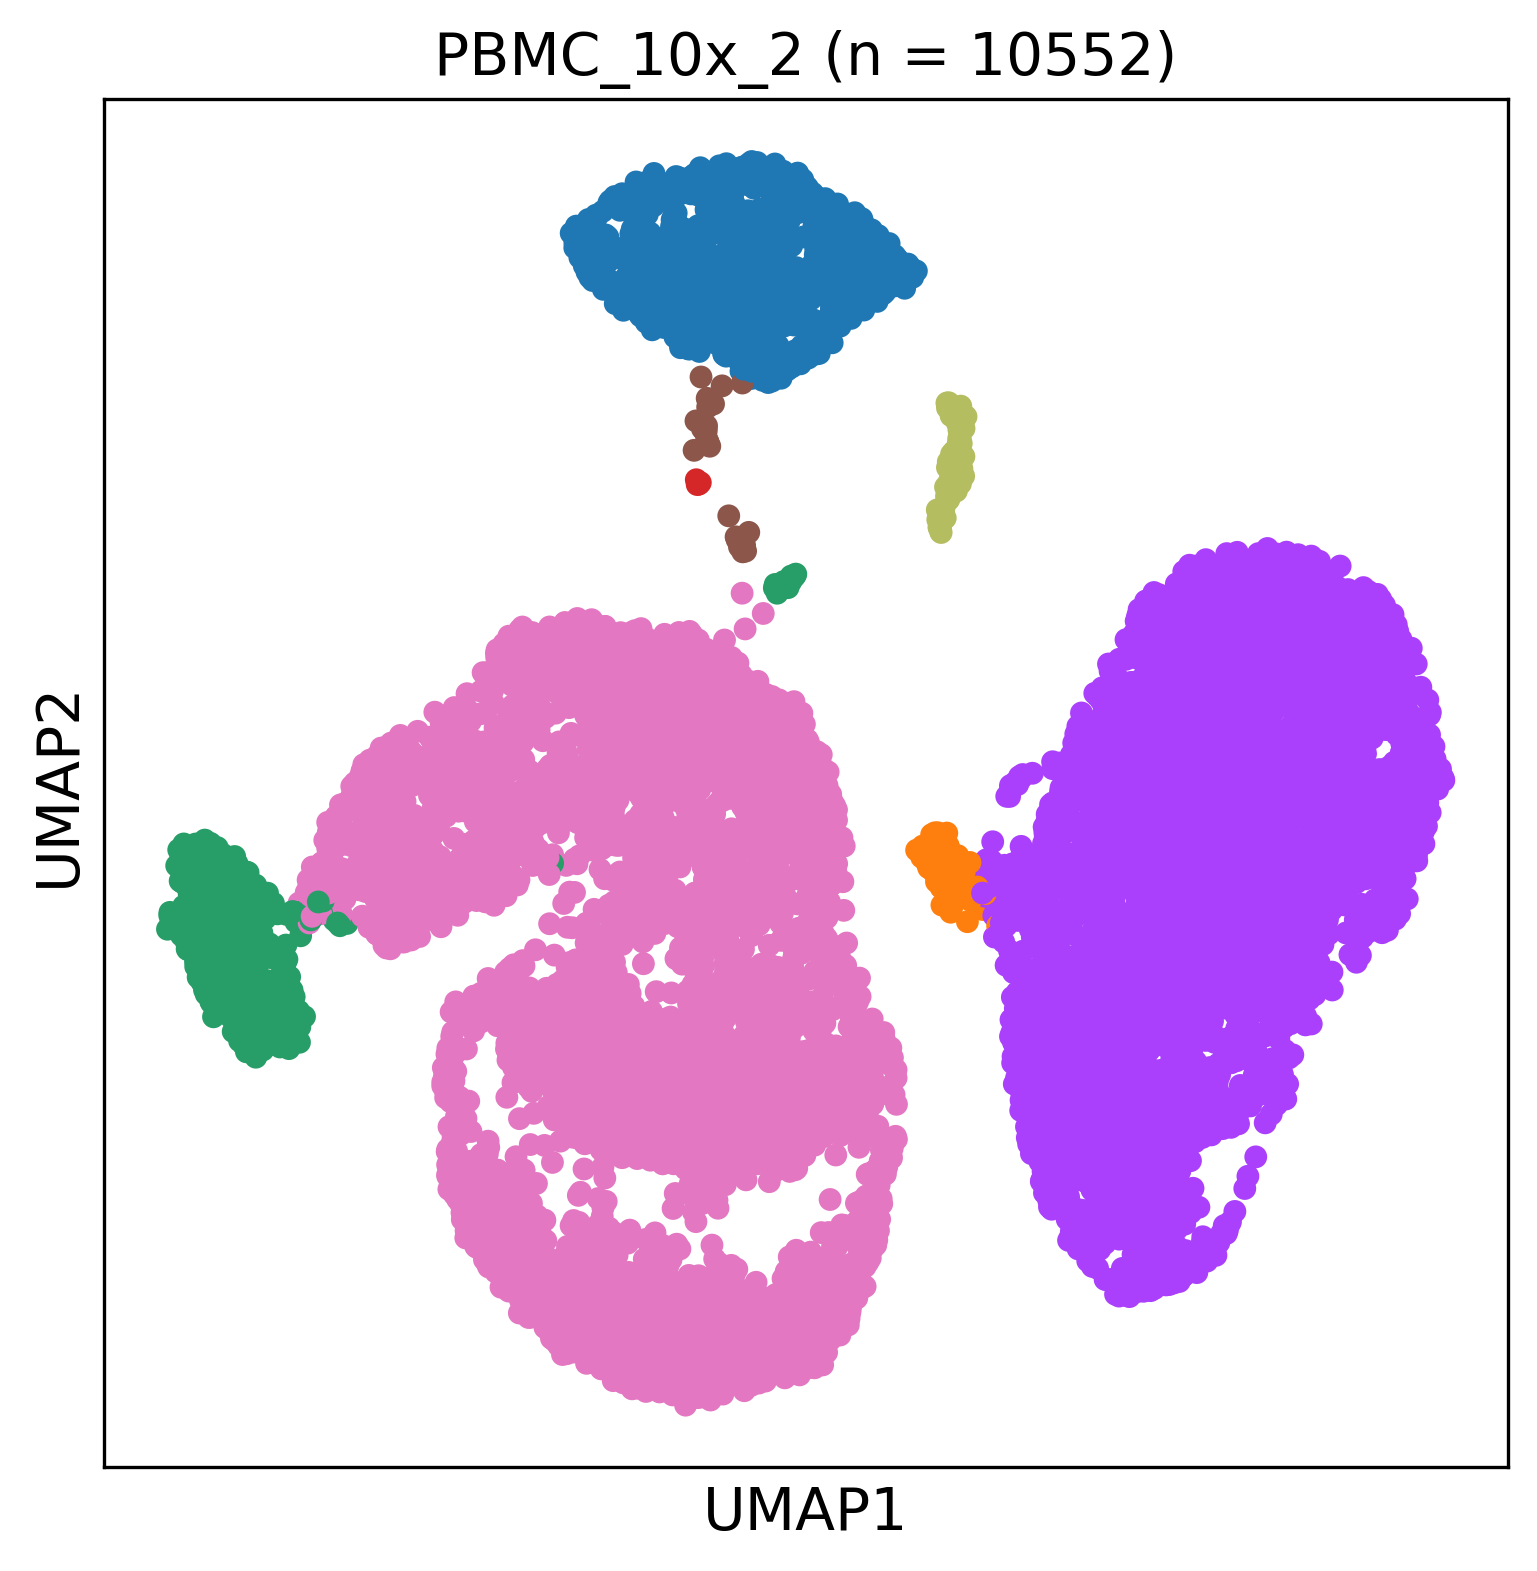
\includegraphics[width=0.25\textwidth]{images/clusterings/PBMC_10x_2.png} &
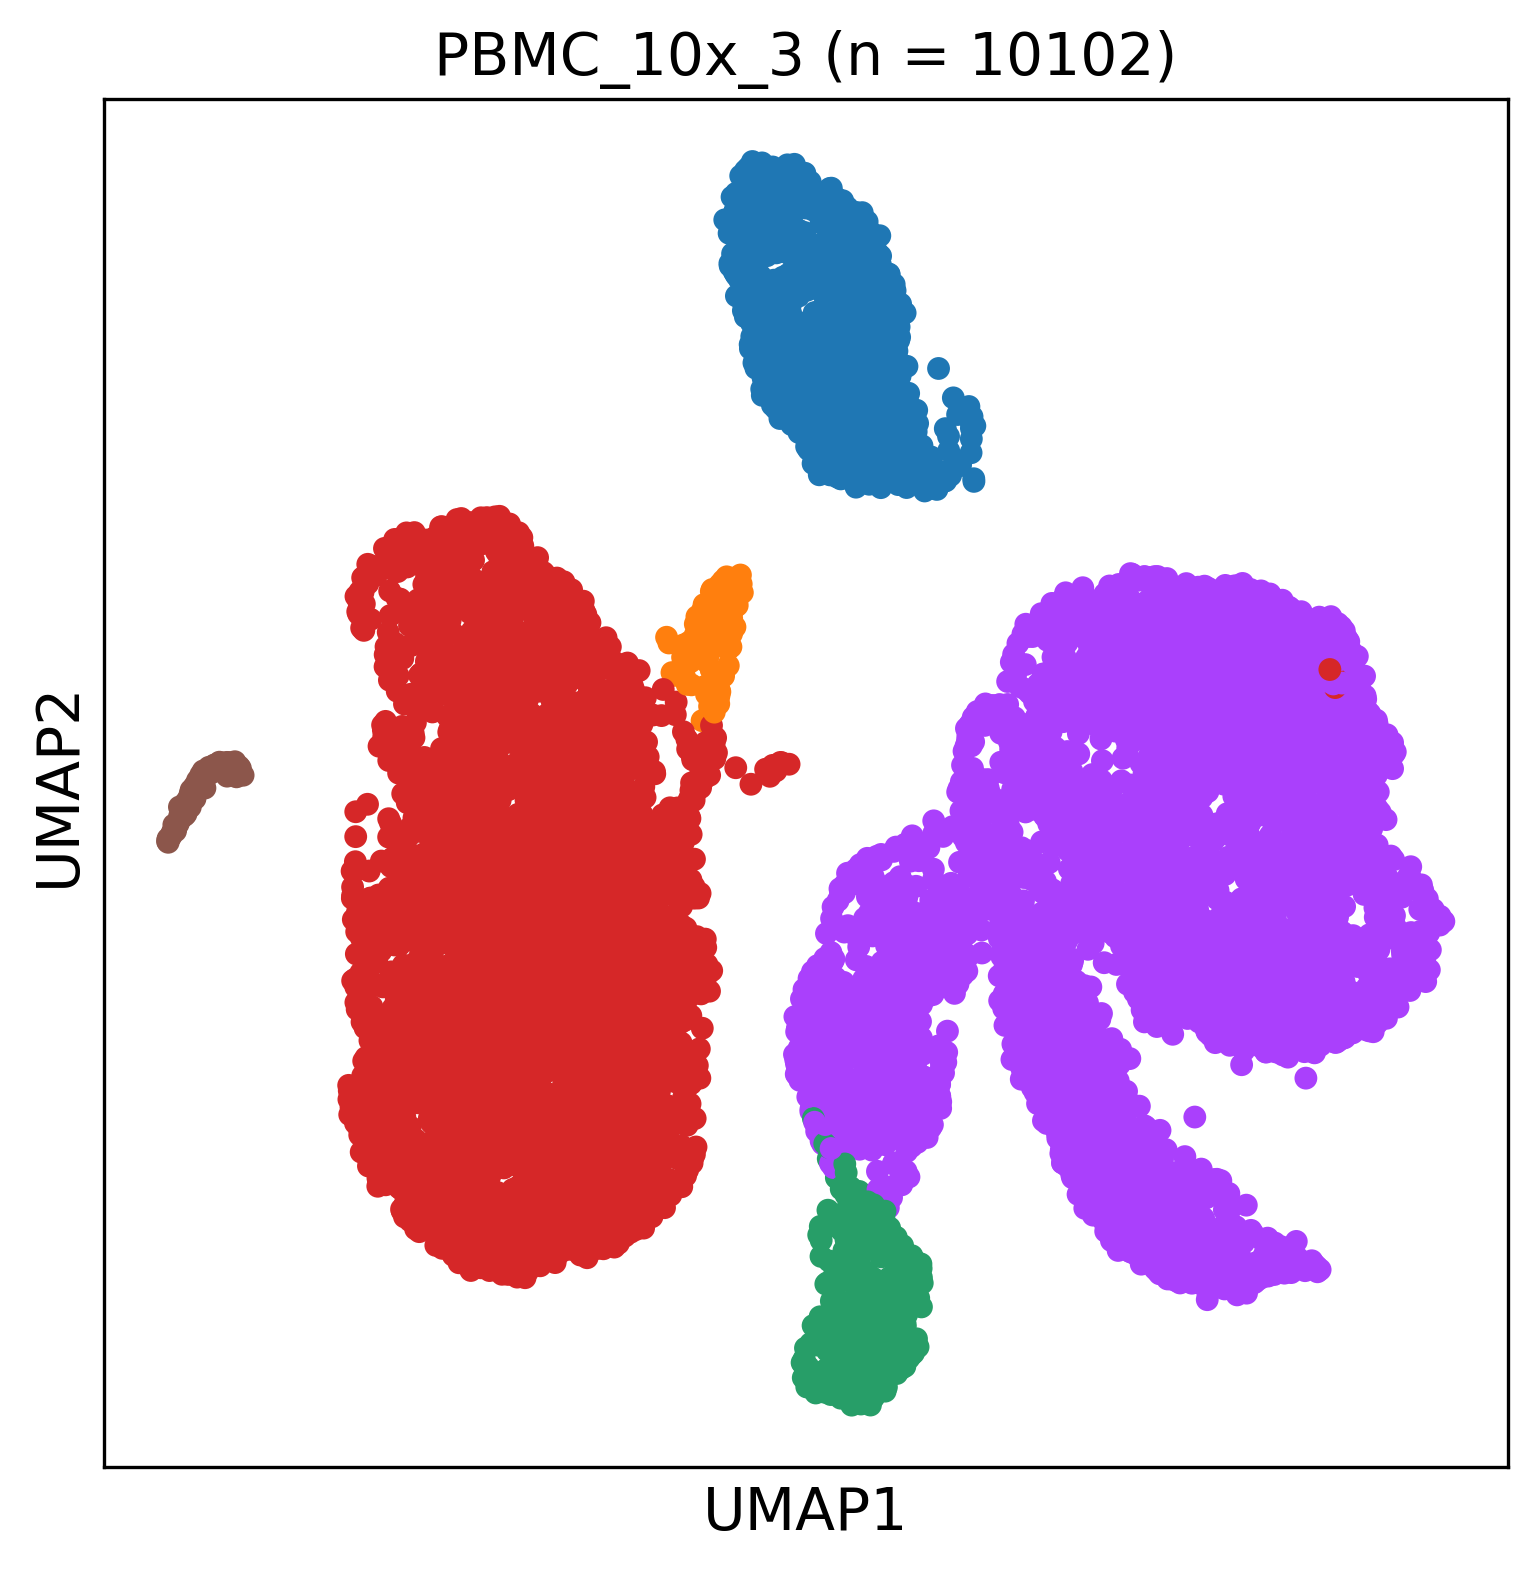
\includegraphics[width=0.25\textwidth]{images/clusterings/PBMC_10x_3.png} \\
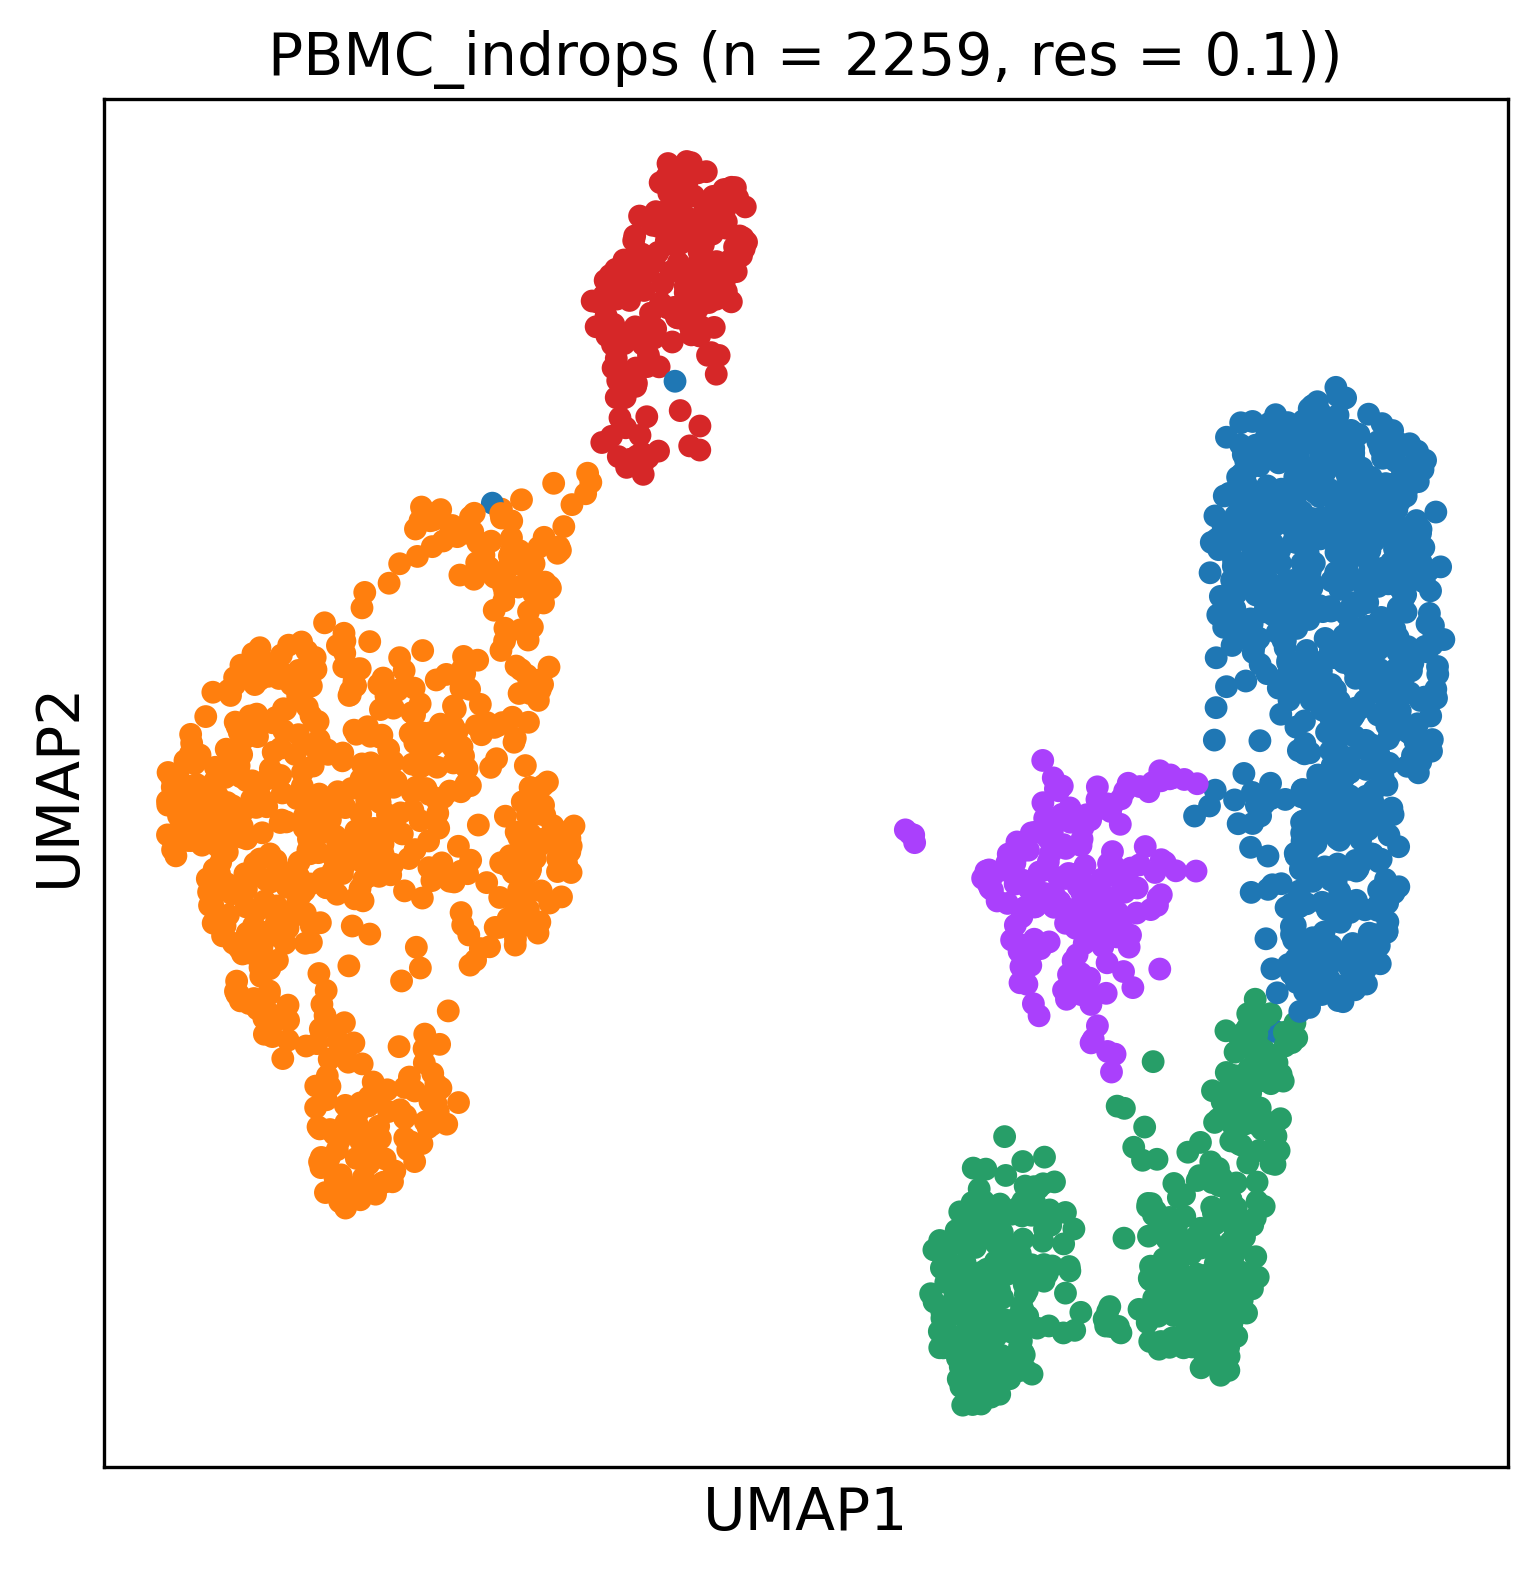
\includegraphics[width=0.25\textwidth]{images/clusterings/PBMC_indrops.png} &
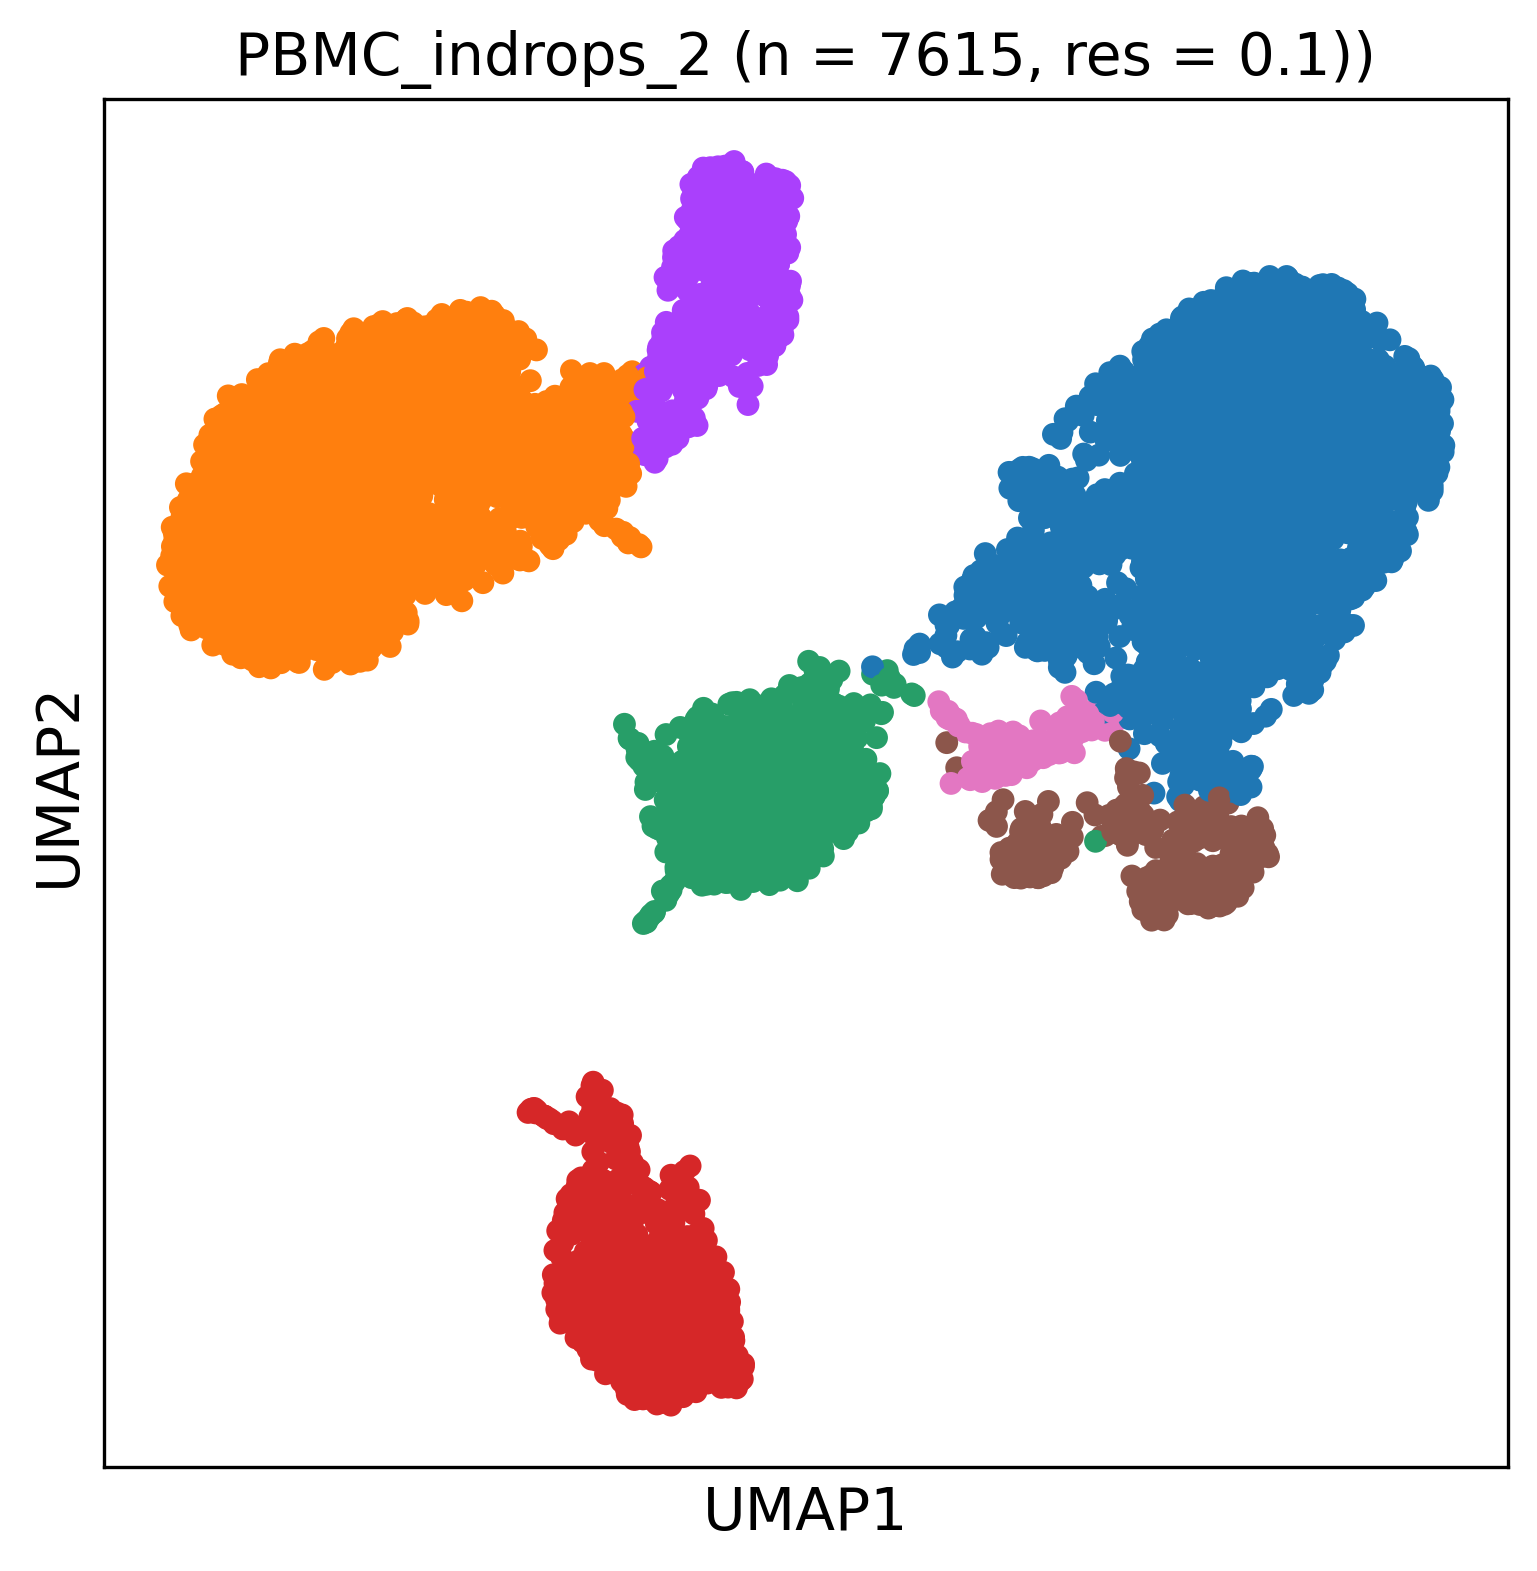
\includegraphics[width=0.25\textwidth]{images/clusterings/PBMC_indrops_2.png} &
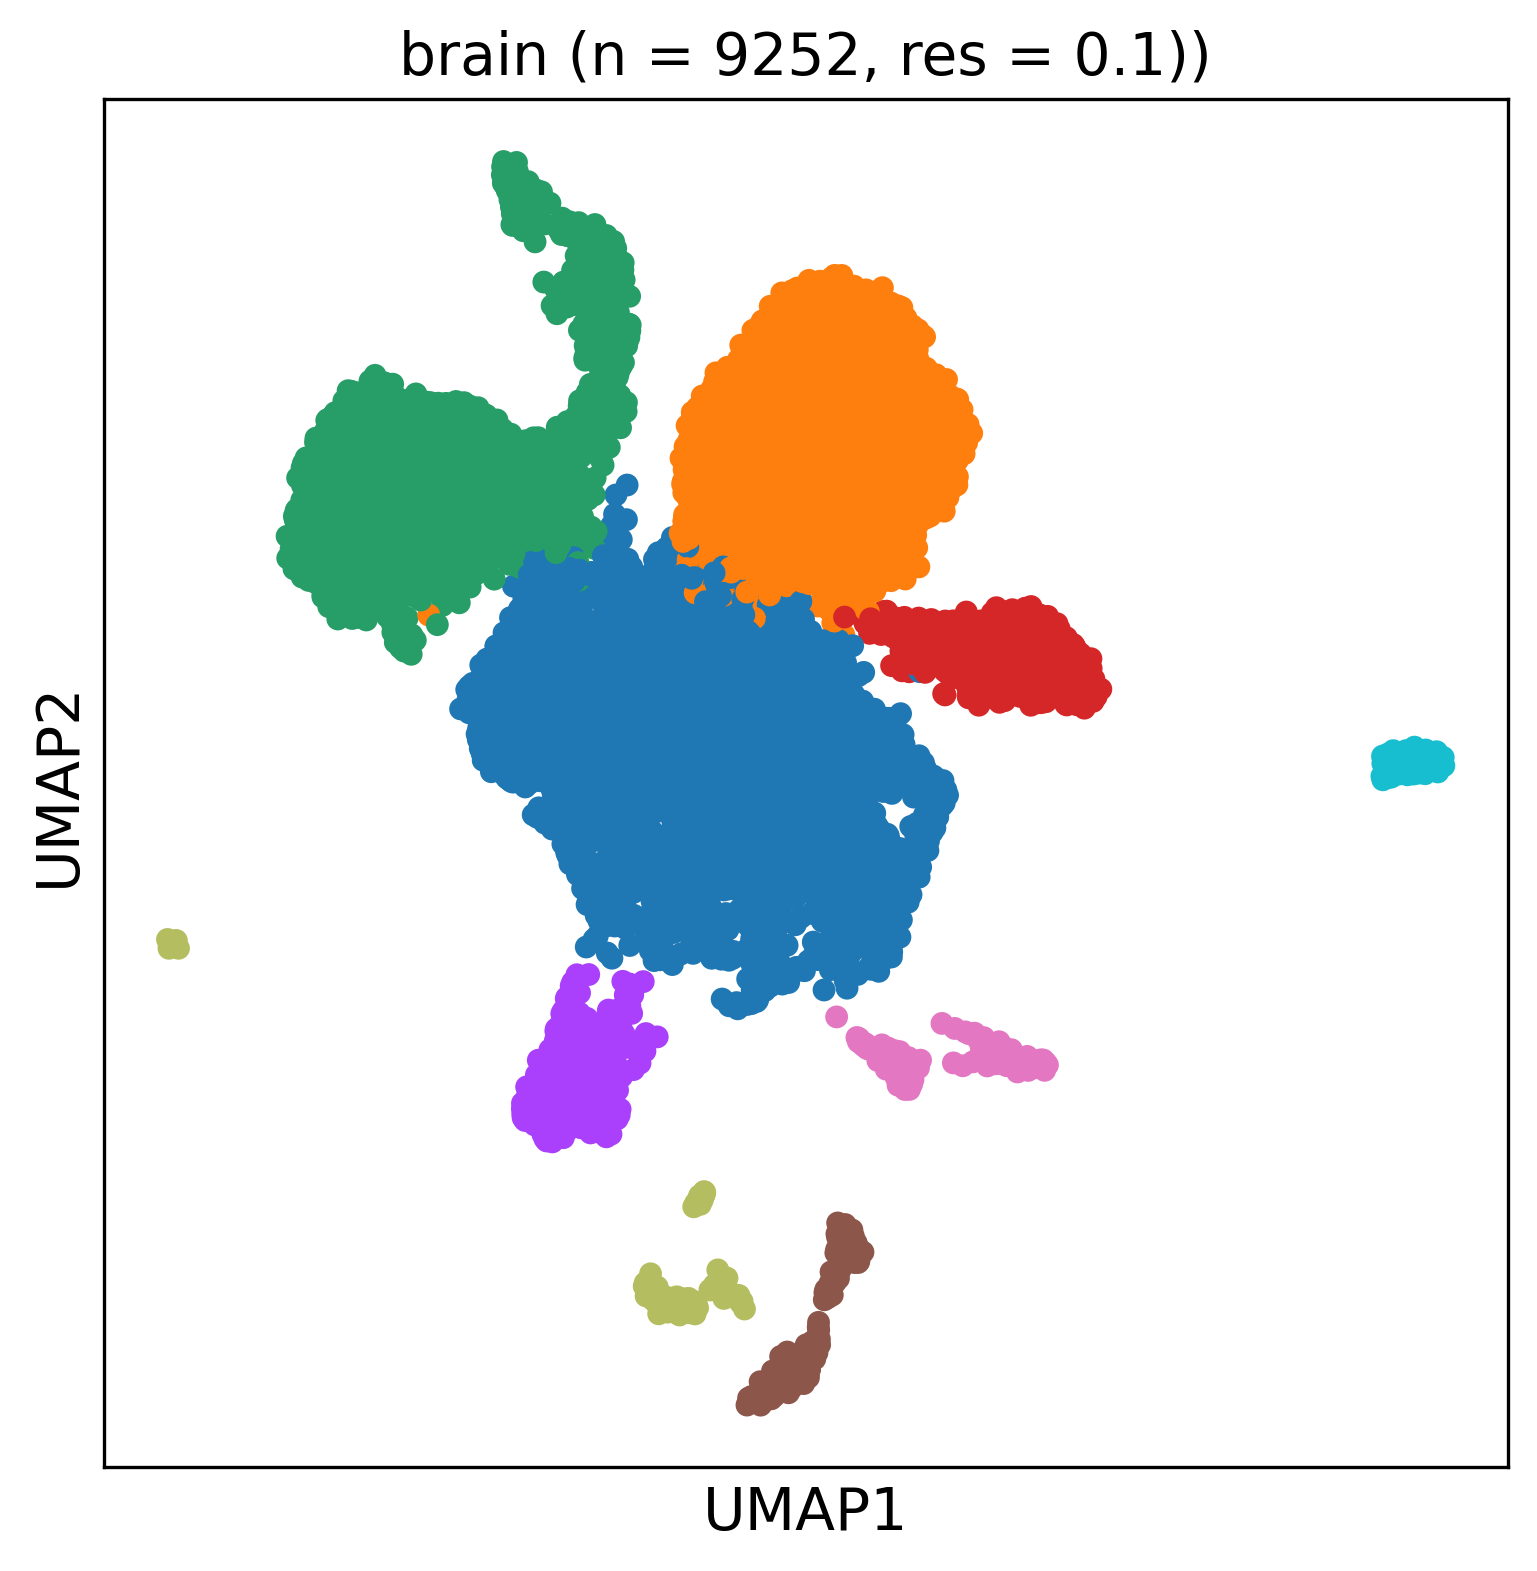
\includegraphics[width=0.25\textwidth]{images/clusterings/brain.png} \\
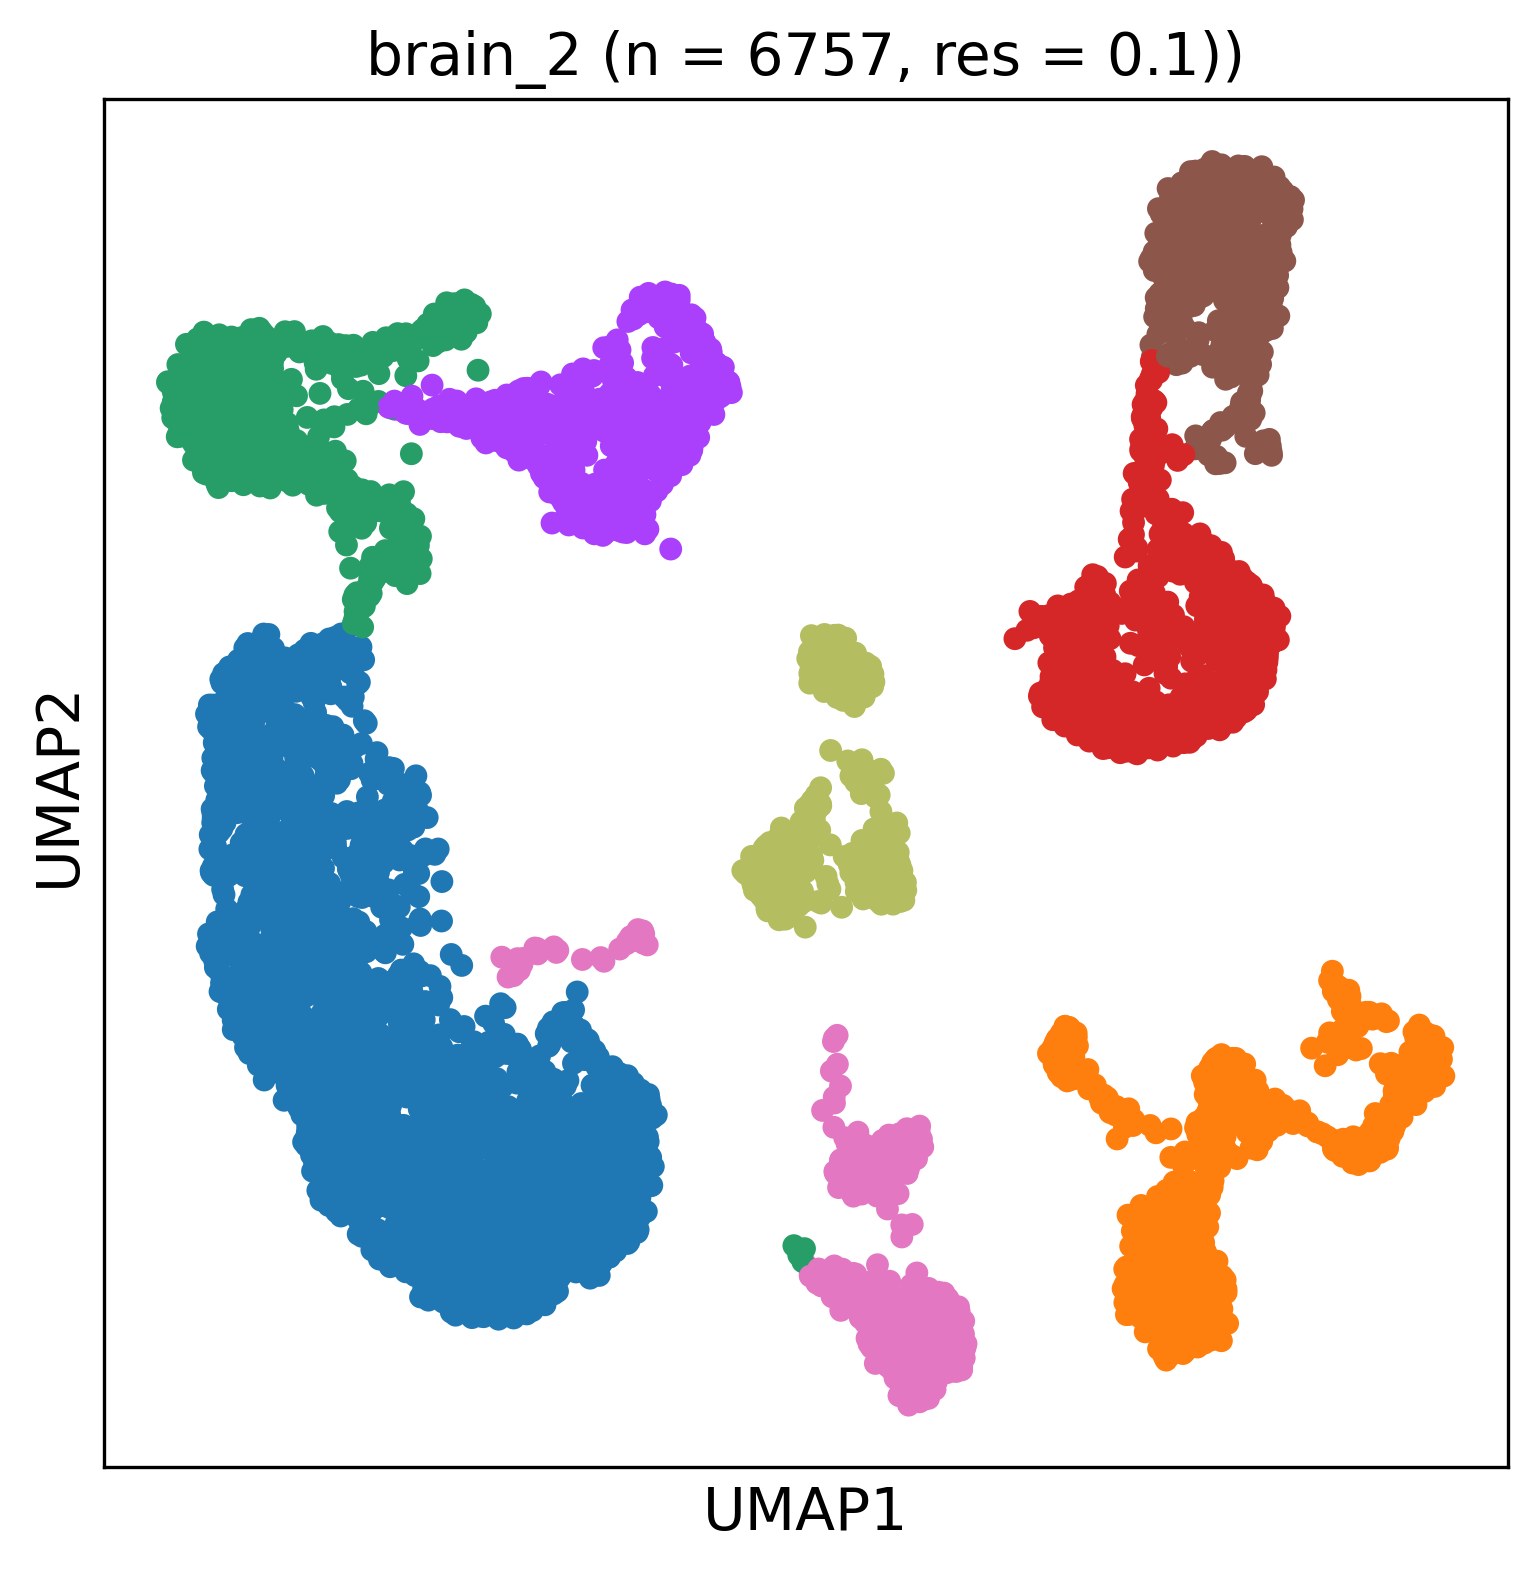
\includegraphics[width=0.25\textwidth]{images/clusterings/brain_2.png} &
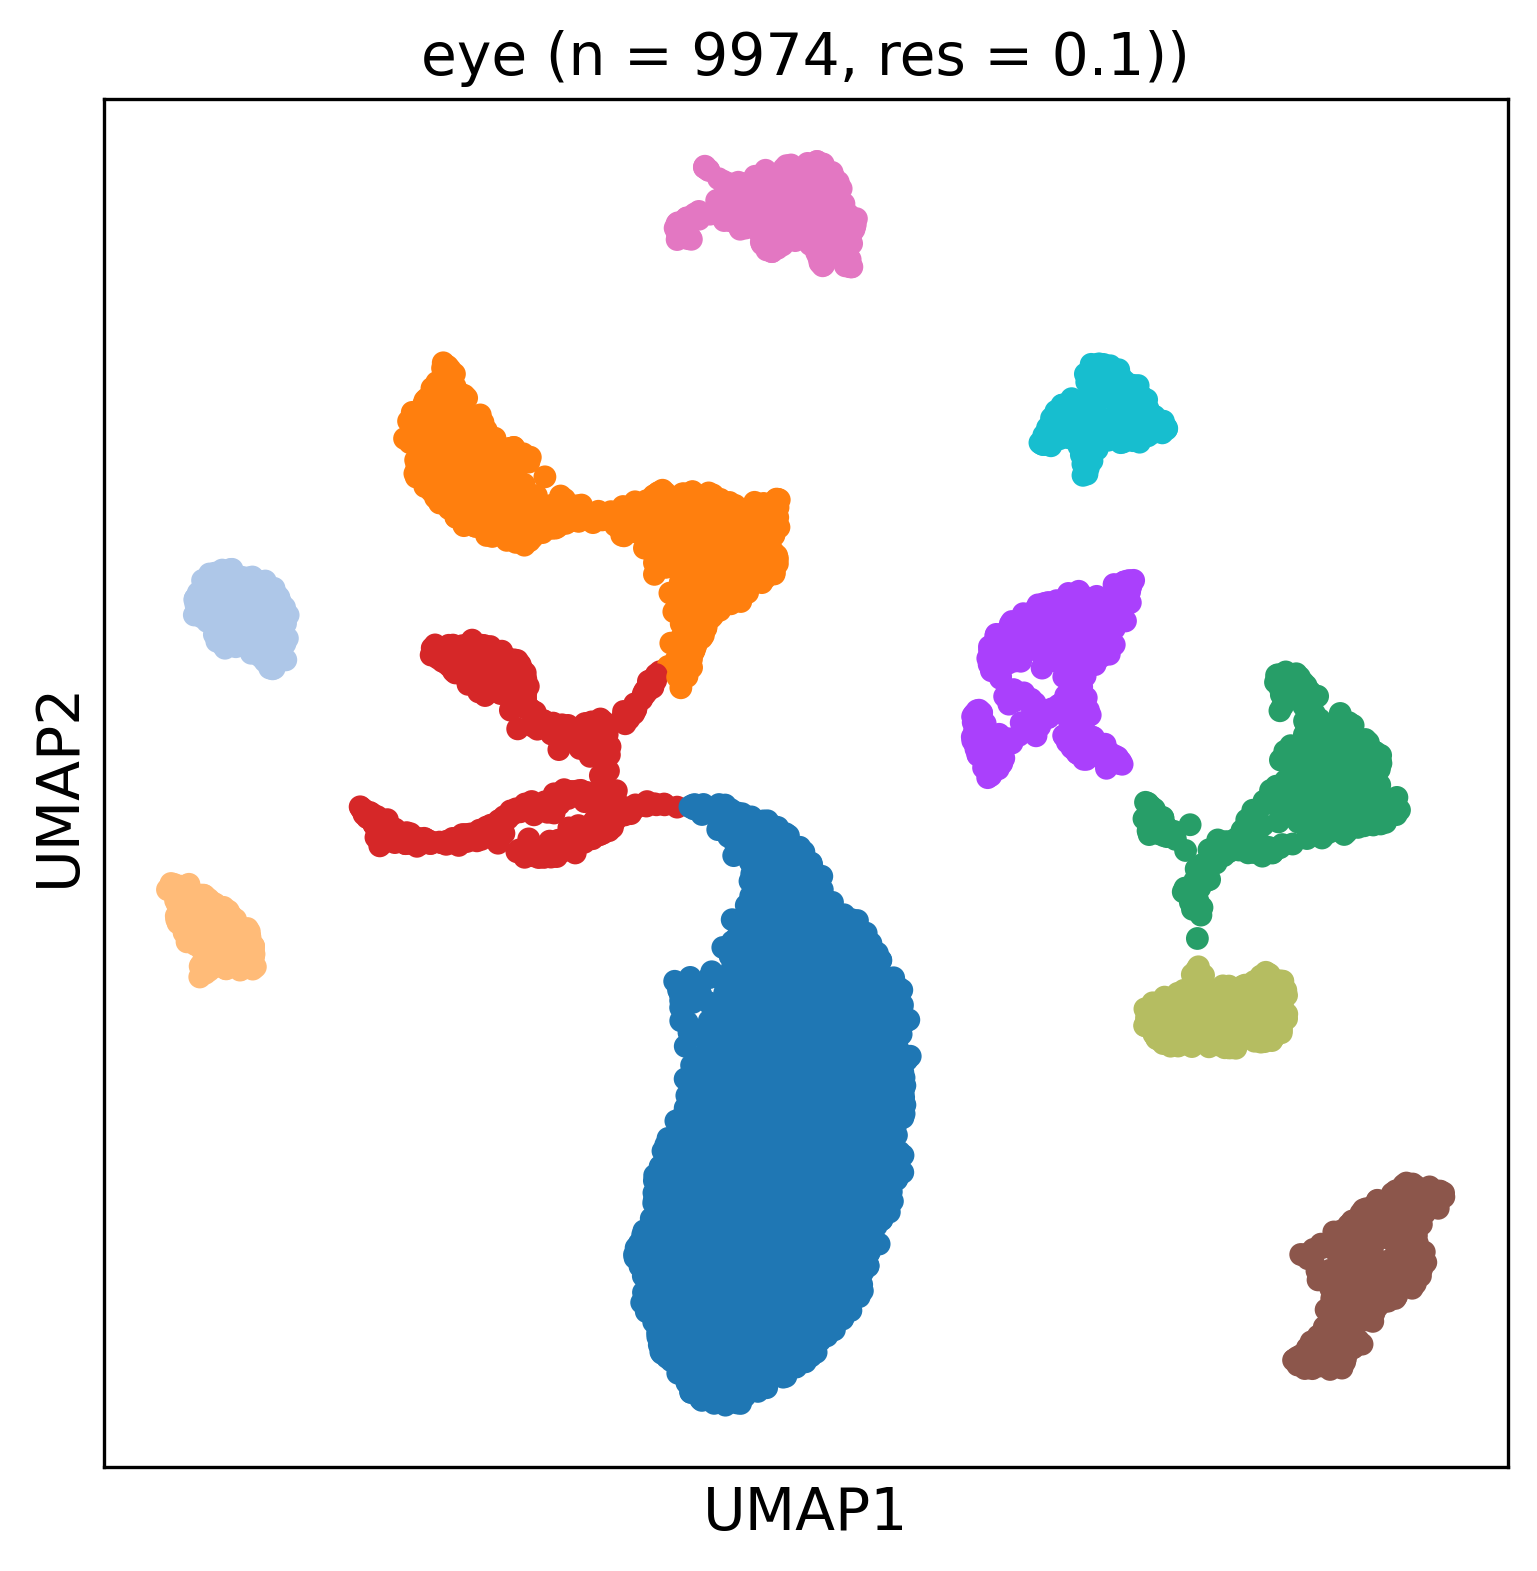
\includegraphics[width=0.25\textwidth]{images/clusterings/eye.png} &
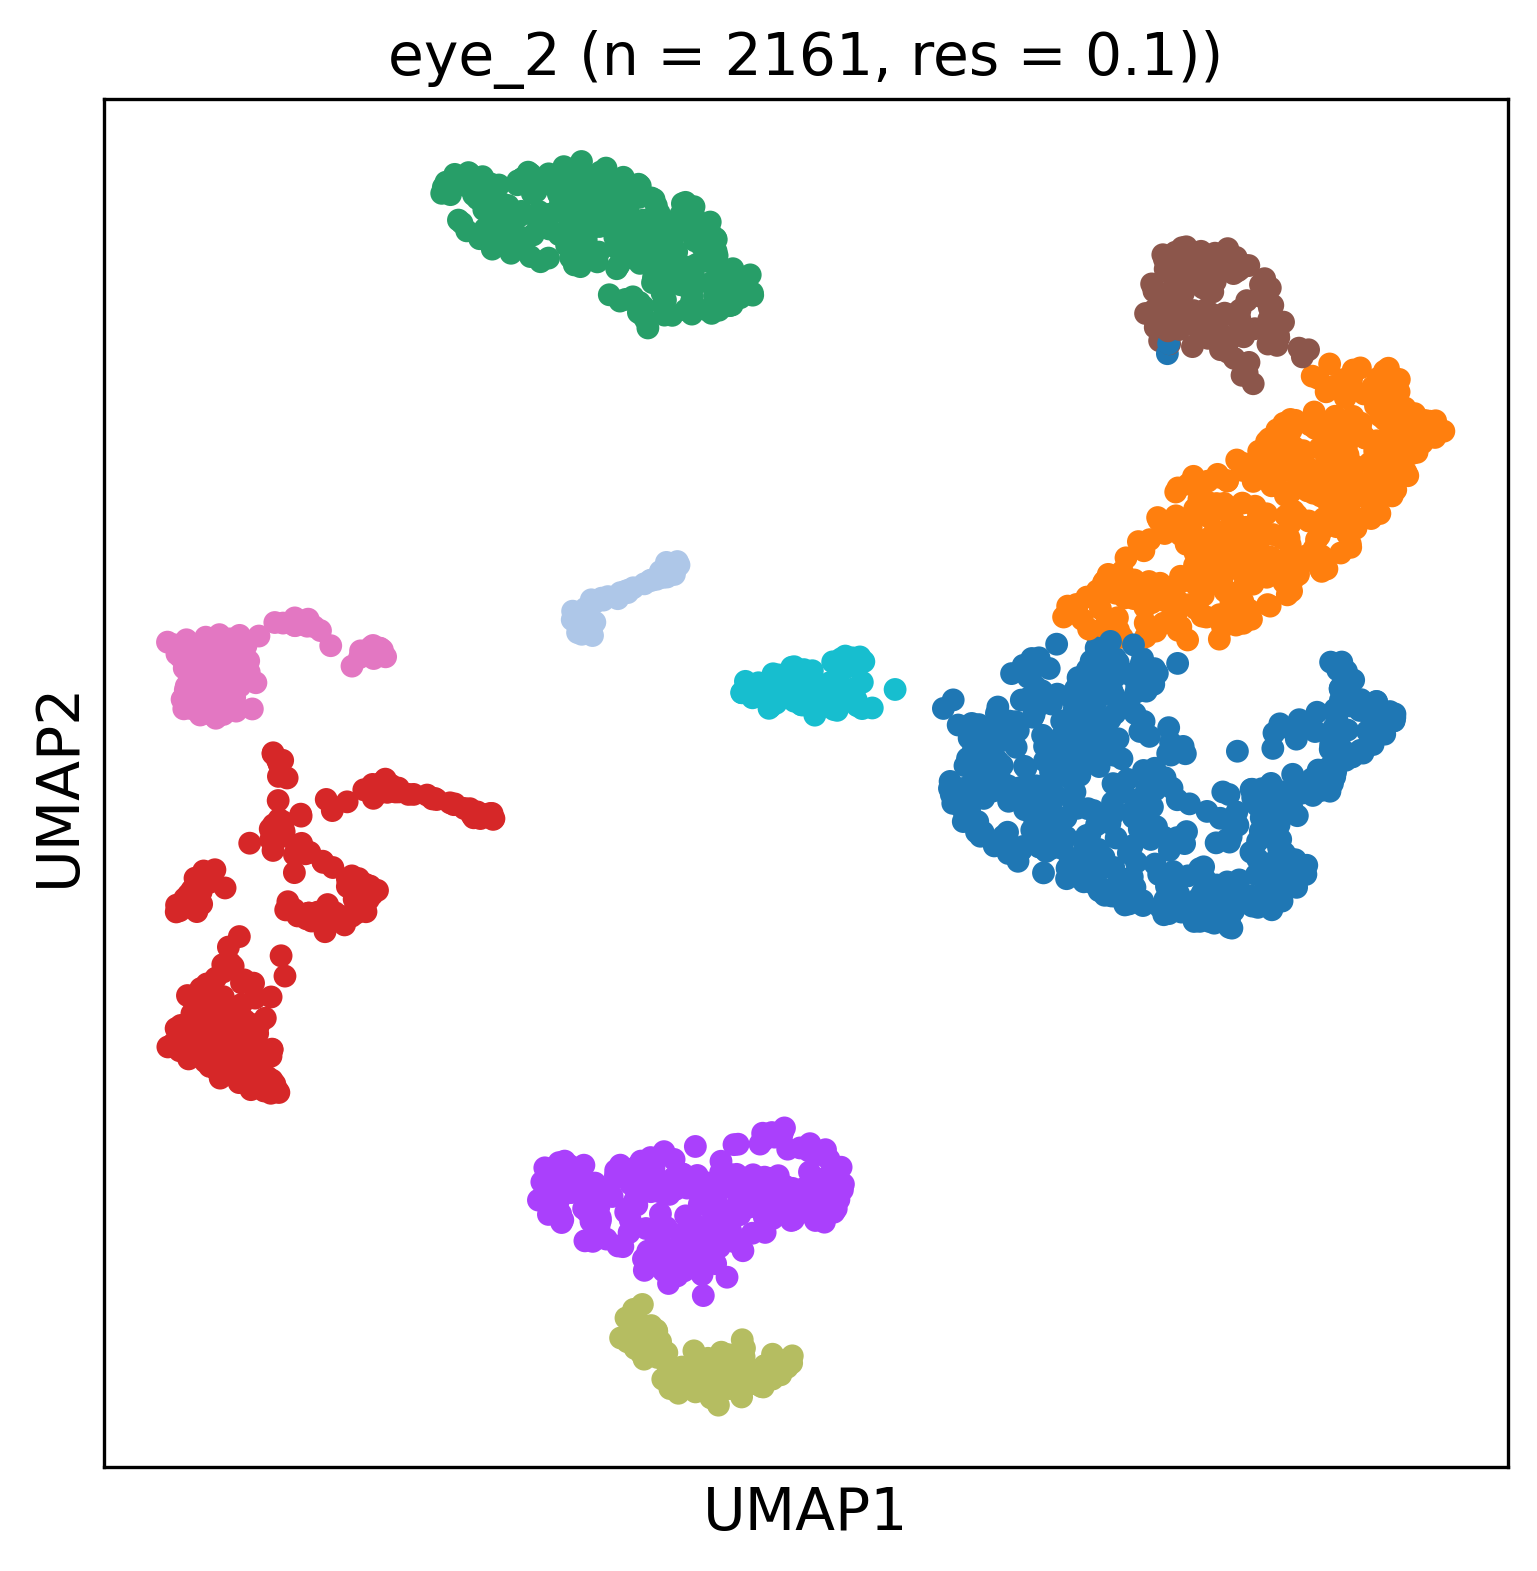
\includegraphics[width=0.25\textwidth]{images/clusterings/eye_2.png} \\
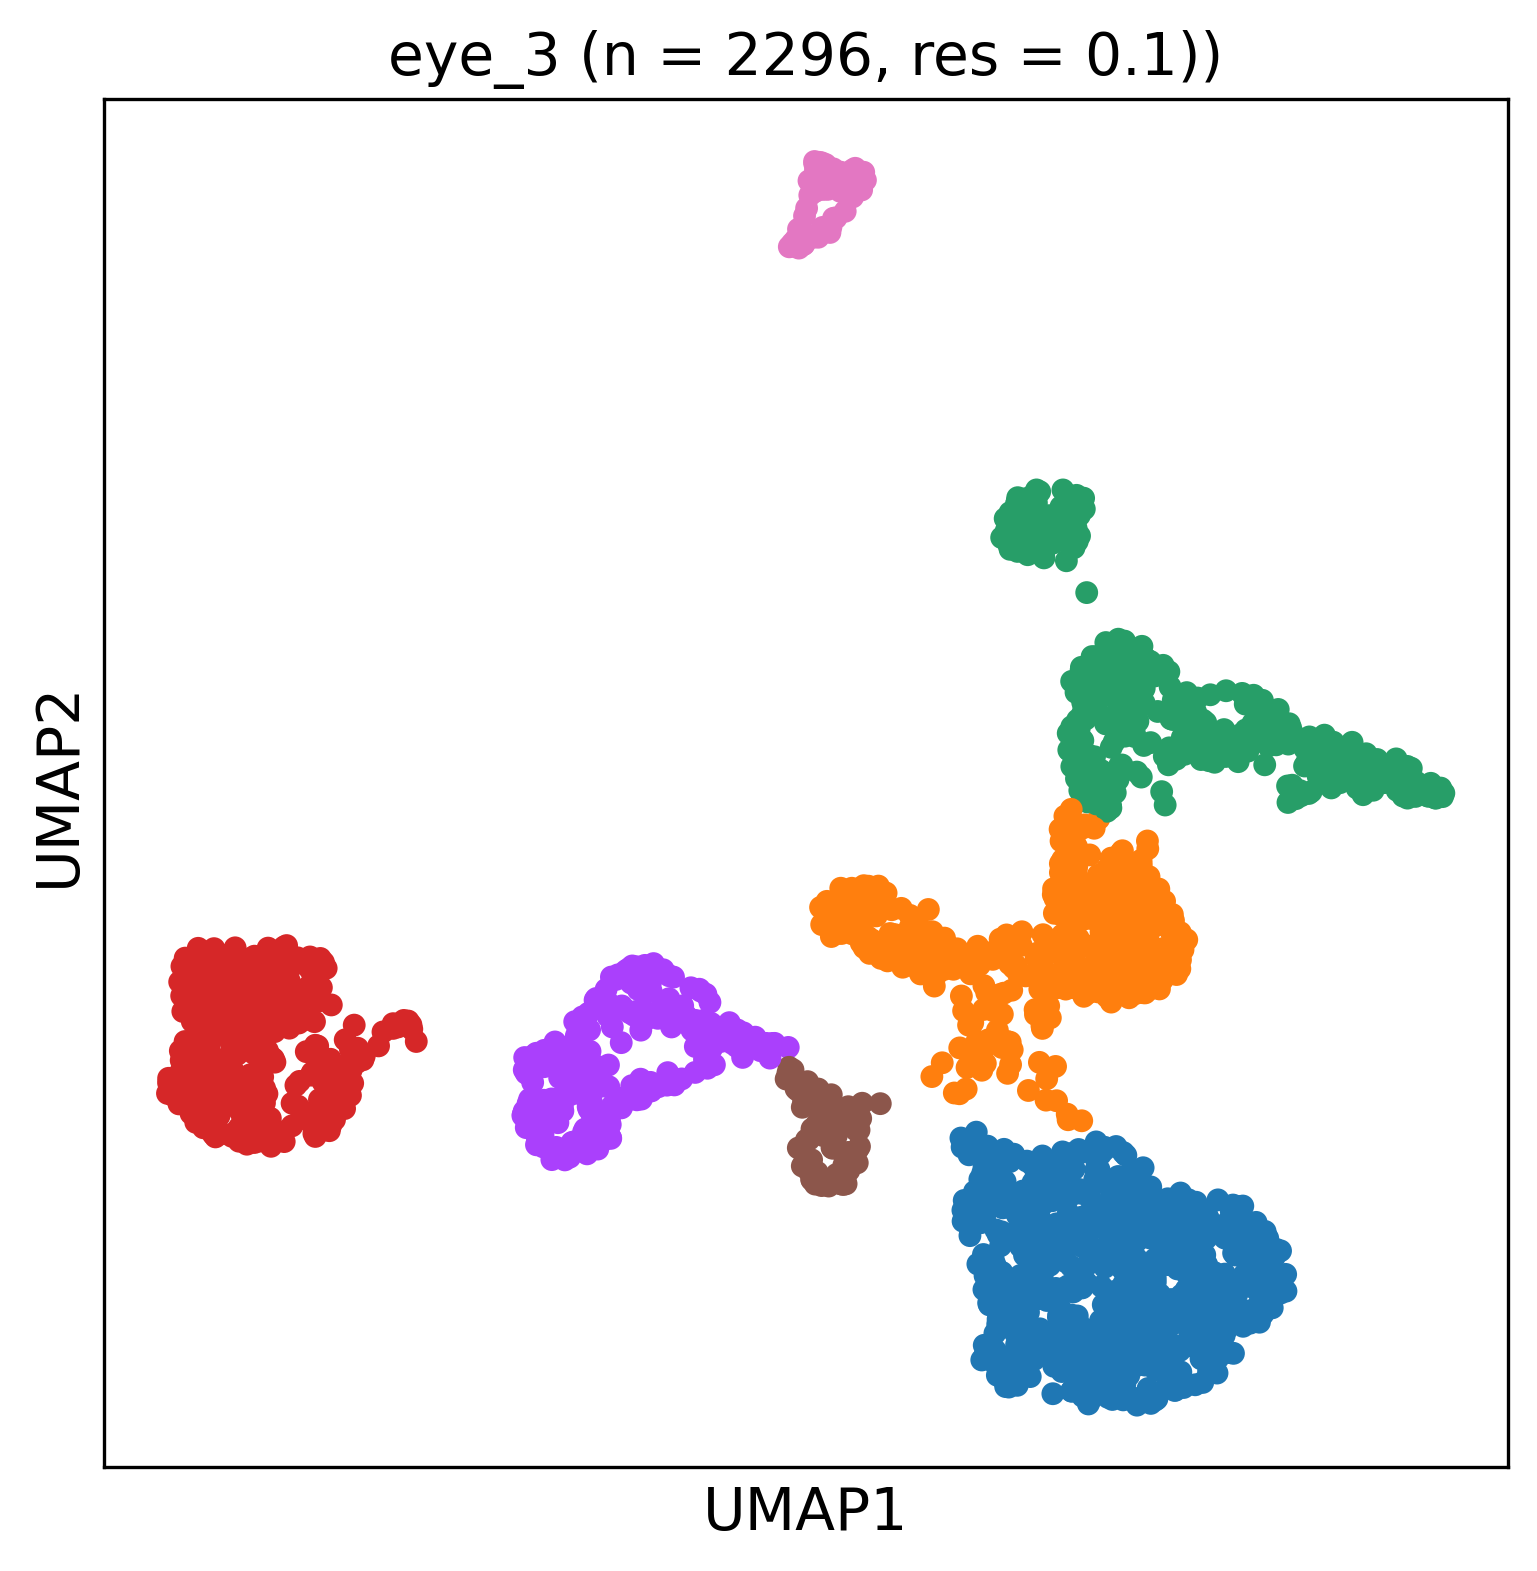
\includegraphics[width=0.25\textwidth]{images/clusterings/eye_3.png} &
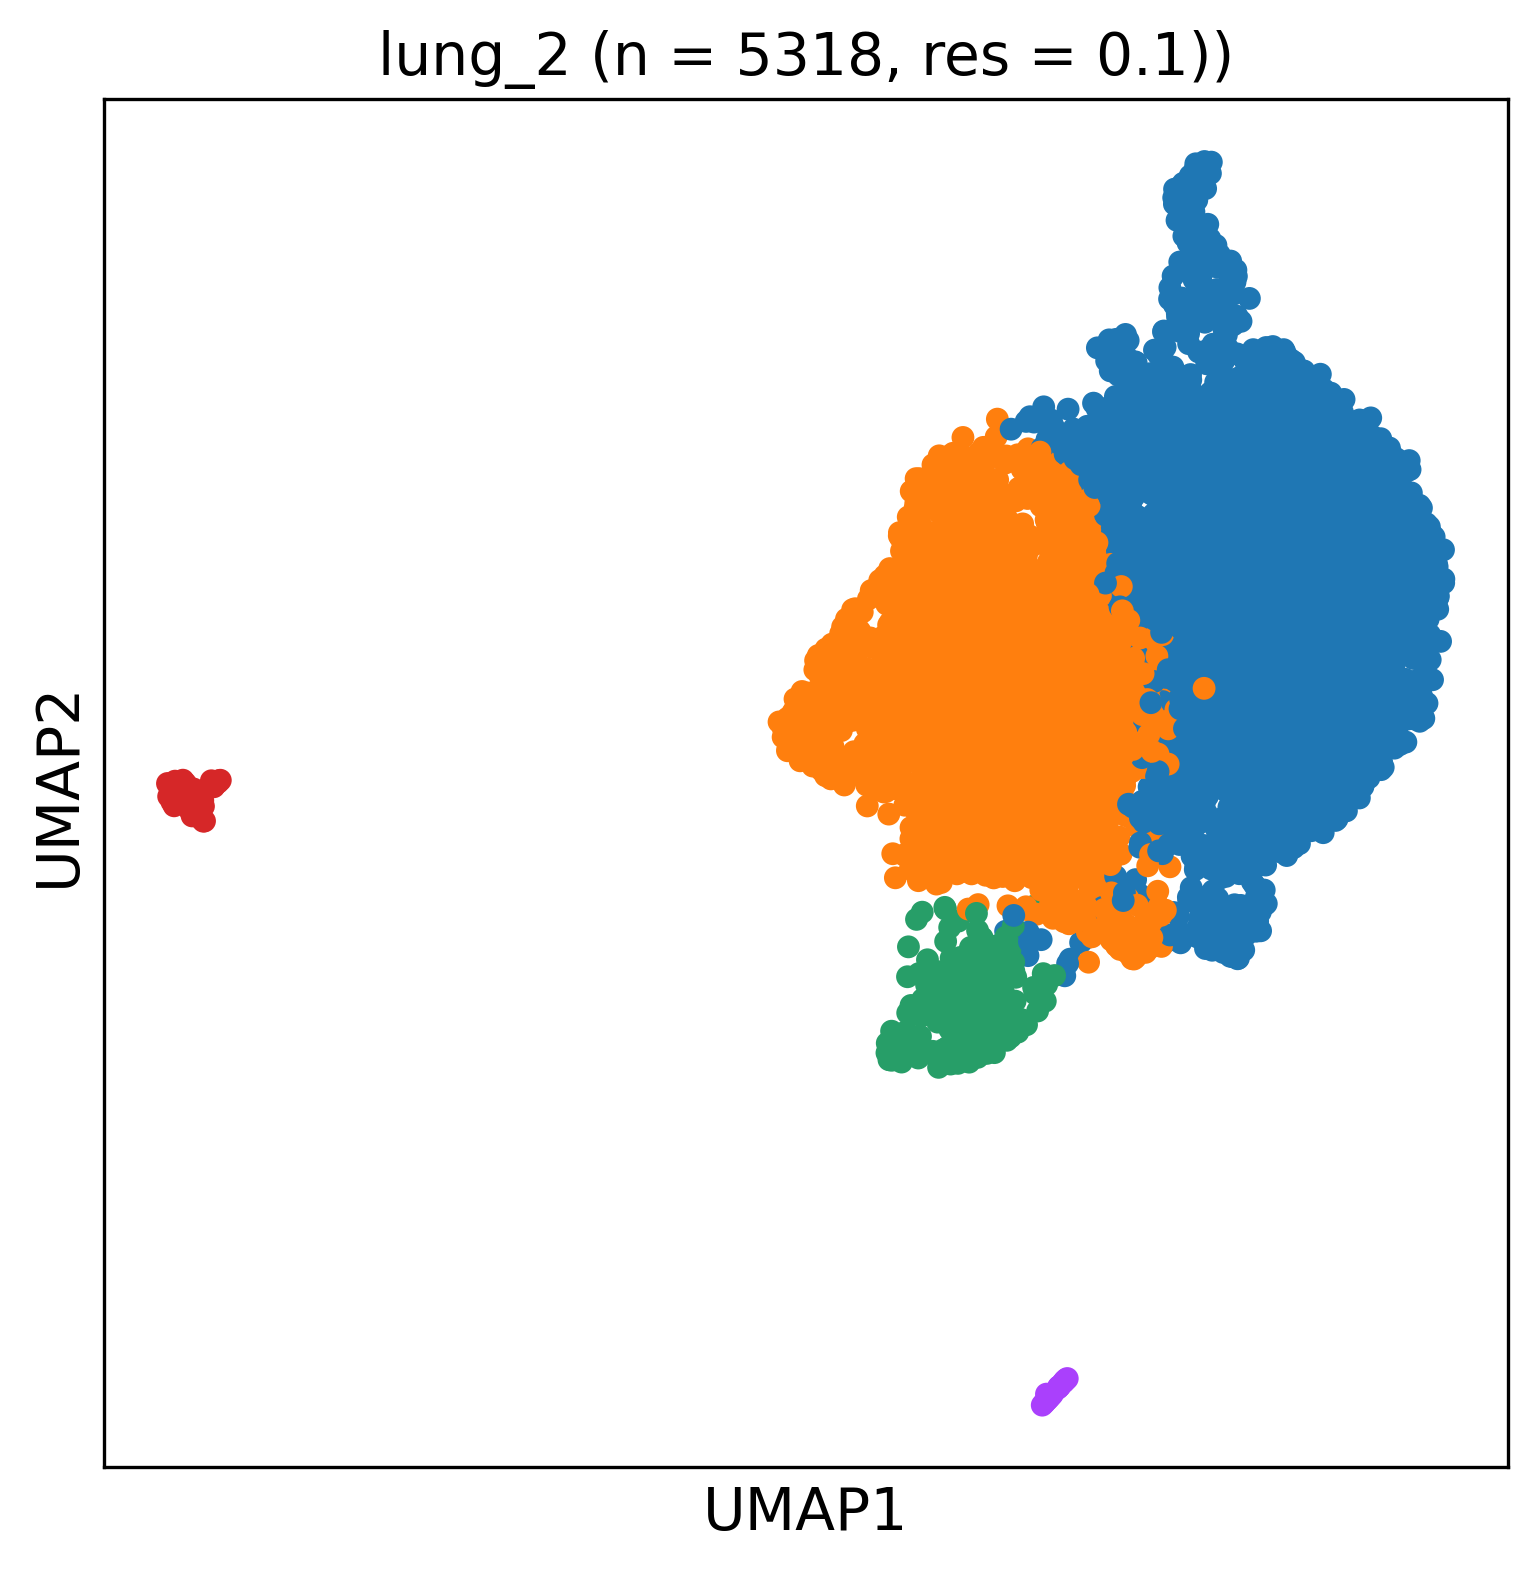
\includegraphics[width=0.25\textwidth]{images/clusterings/lung_2.png} &
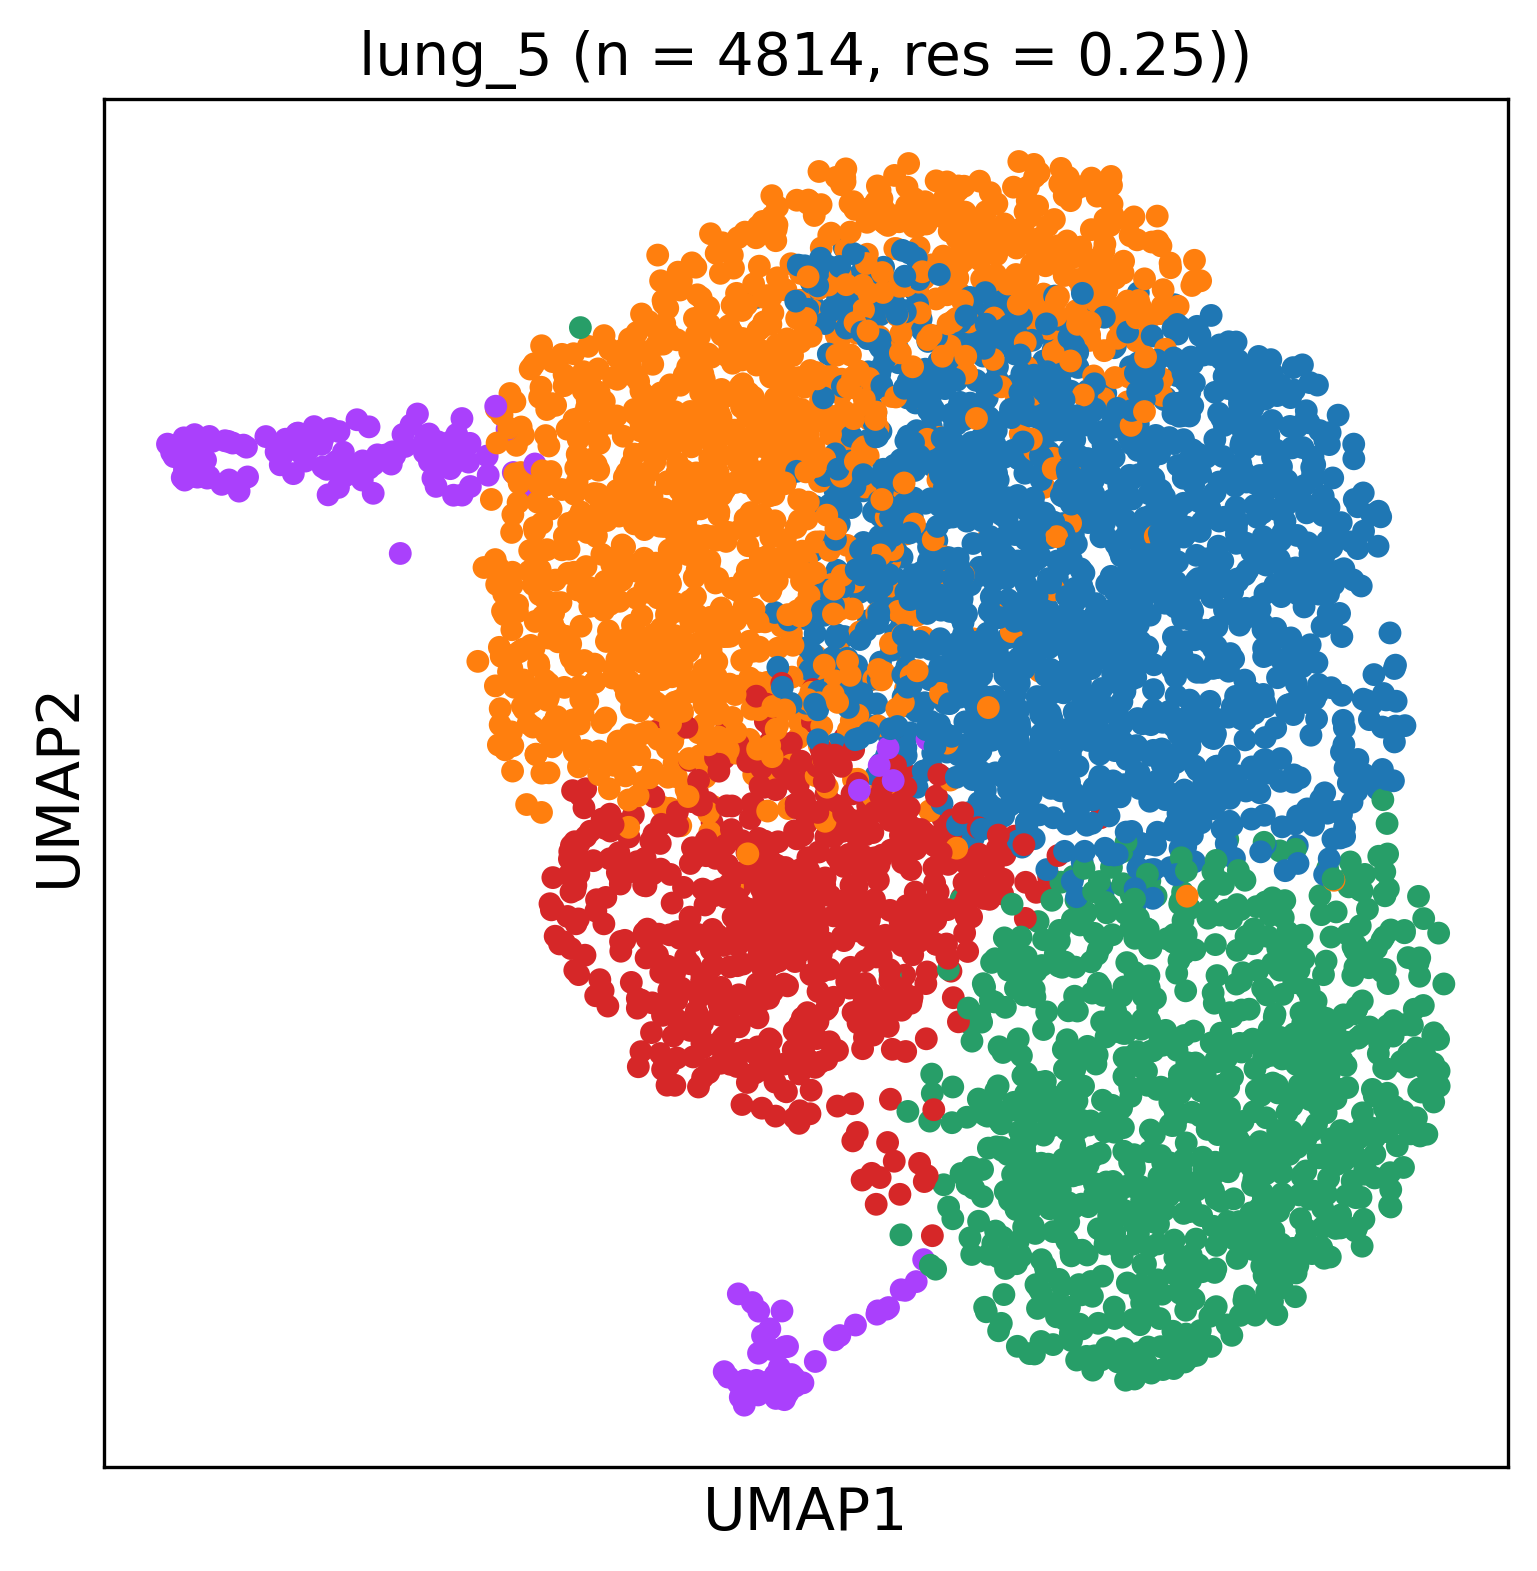
\includegraphics[width=0.25\textwidth]{images/clusterings/lung_5.png} \\
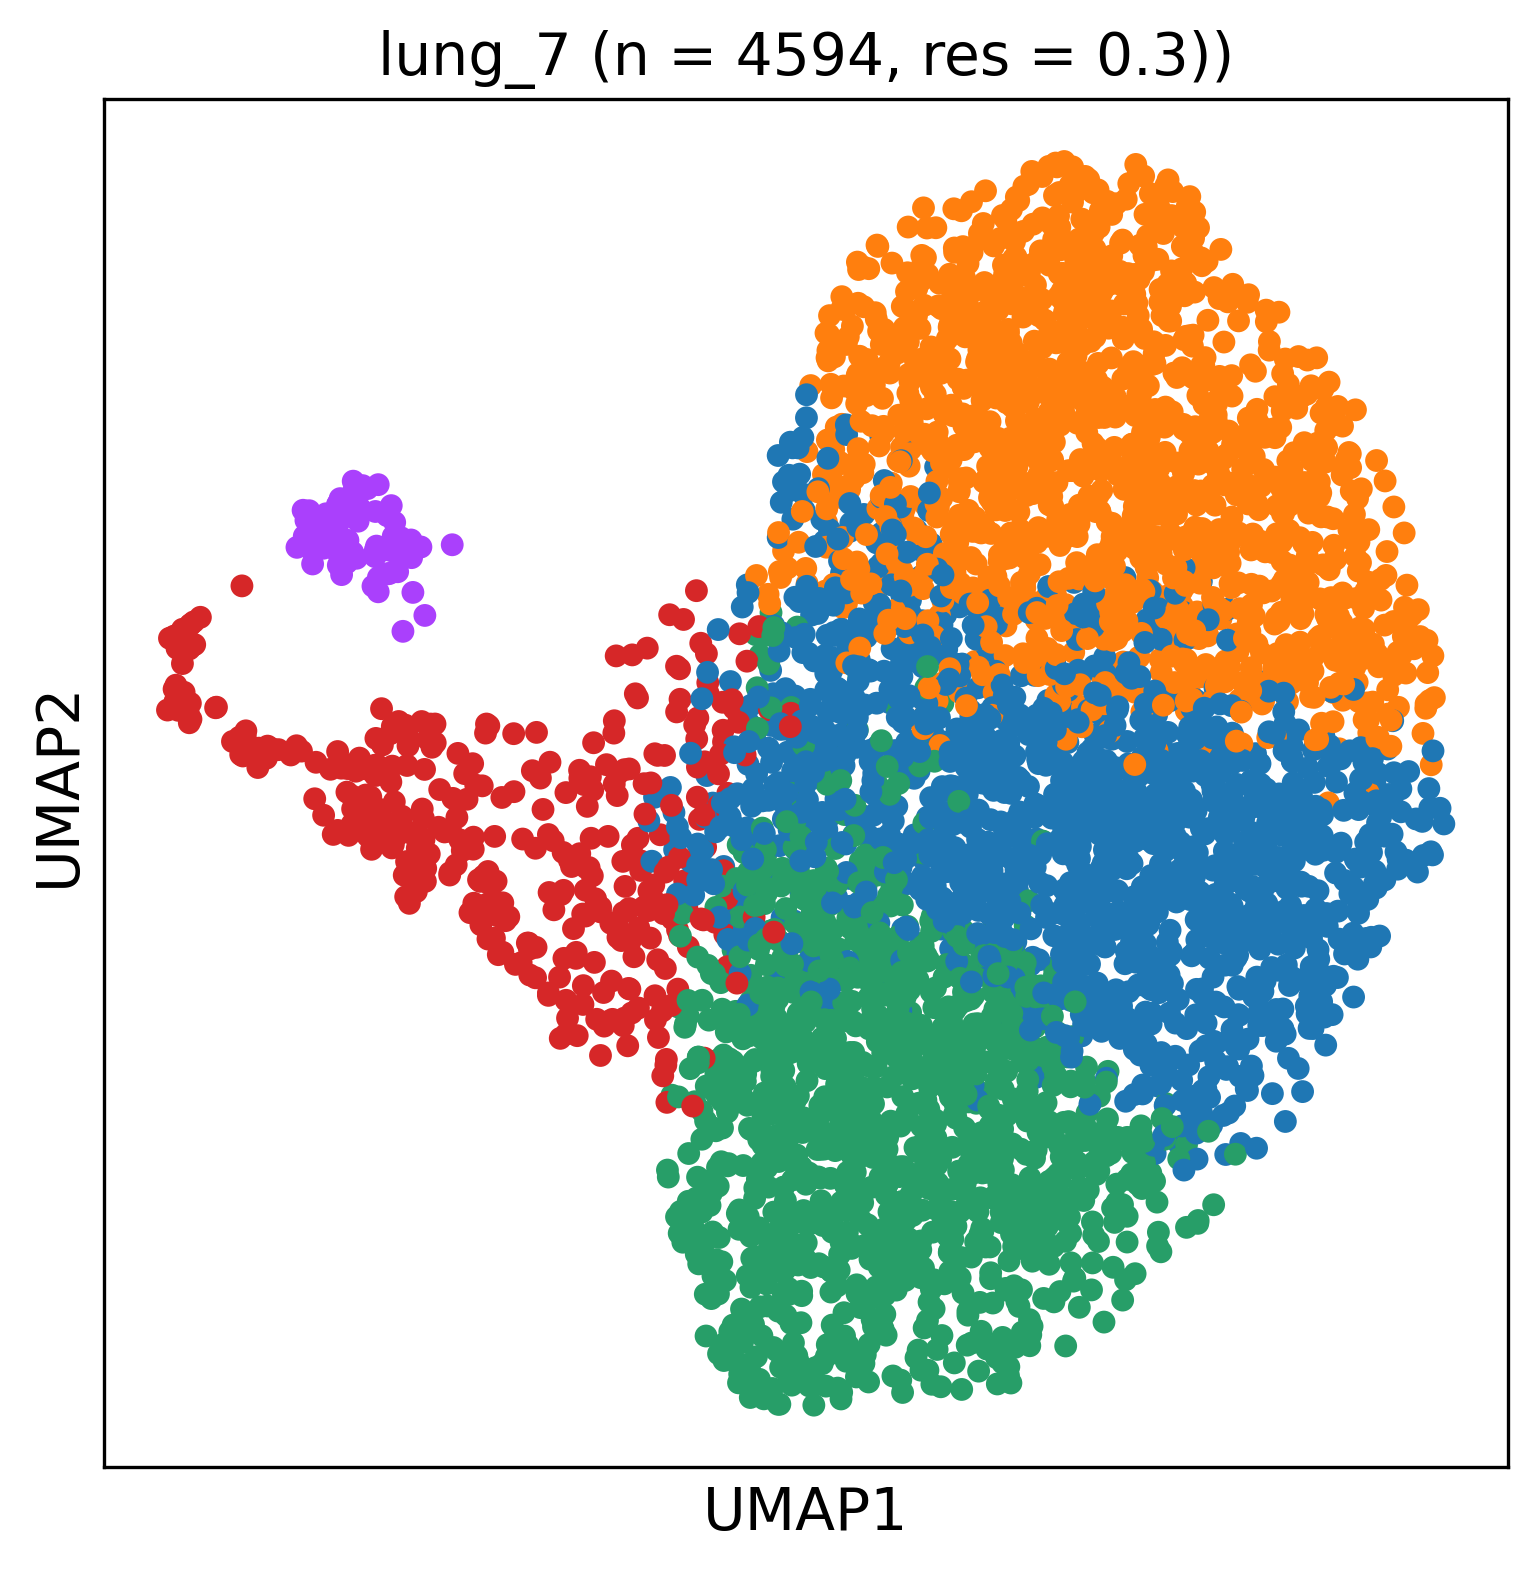
\includegraphics[width=0.25\textwidth]{images/clusterings/lung_7.png} &
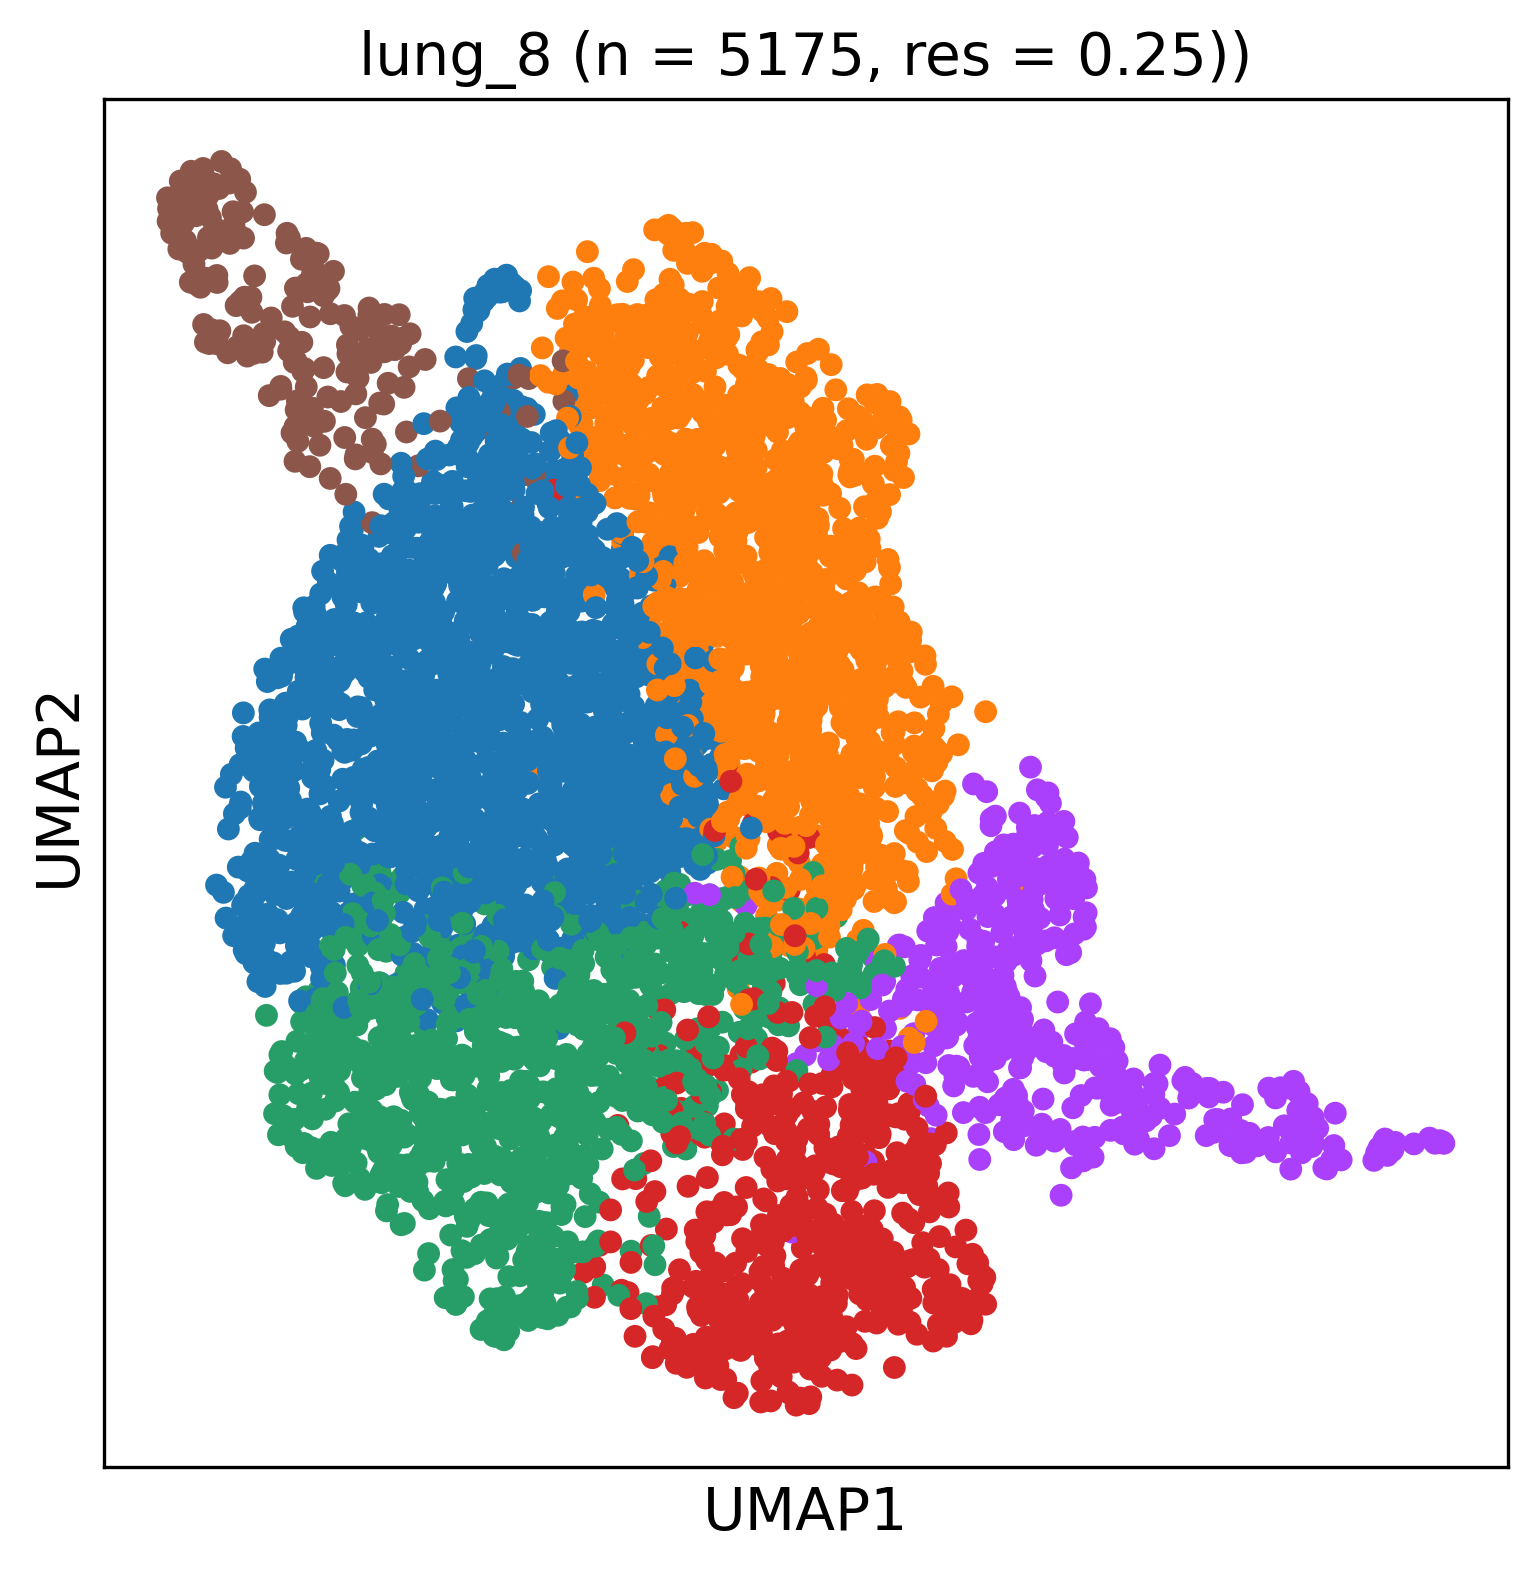
\includegraphics[width=0.25\textwidth]{images/clusterings/lung_8.png} &
\\
\end{tabular}
\caption{Clusterings of datasets. 'n' stands for number of cells in the plot, 'res' for the resolution parameter of leiden algorithm.
\textit{PBMC\_10x} samples are colored by CellTypist annotations.}
\label{fig:clusterings}
\end{figure}
